\documentclass[11pt, oneside]{report}
\usepackage[a4paper,top=3cm,bottom=3cm,left=3cm,right=2cm]{geometry}
\usepackage[utf8]{inputenc}
\usepackage[T1]{fontenc}
\usepackage{graphicx}
\usepackage{url}
\usepackage{float}
\usepackage{titlesec}

\usepackage[hidelinks,breaklinks]{hyperref}
\usepackage[slovak]{babel} % vypnite pre prace v anglictine
\usepackage{listings}\usepackage{graphicx}
\graphicspath{ {images/} }

\usepackage{color}
\definecolor{gray}{rgb}{0.4,0.4,0.4}
\definecolor{darkblue}{rgb}{0.0,0.0,0.6}
\definecolor{cyan}{rgb}{0.0,0.6,0.6}
\definecolor{orange}{rgb}{1,0.45,0}

\lstset{
  basicstyle=\ttfamily,
  columns=fullflexible,
  showstringspaces=false,
  commentstyle=\color{gray}\upshape
}

\lstdefinelanguage{XML}
{
  morestring=[b]",
  morestring=[s]{>}{<},
  morecomment=[s]{<?}{?>},
  stringstyle=\color{black},
  identifierstyle=\color{darkblue},
  keywordstyle=\color{cyan},
  morekeywords={xmlns,version,type}% list your attributes here
}

\lstdefinelanguage{JavaScript}{
  morekeywords={typeof, new, true, false, catch, function, return, null, catch, switch, var, if, in, while, do, else, case, break},
  morecomment=[s]{/*}{*/},
  morecomment=[l]//,
  morestring=[b]",
  morestring=[b]'
}

\lstdefinelanguage{HTML5}{
		showstringspaces=true,
		keepspaces=true,
        language=html,
        sensitive=true, 
		literate=%
		{@}{{{\color{orange}@}}}1
		{\{}{{{\color{orange}\{}}}1
		{\}}{{{\color{orange}\}}}}1,
        alsoletter={<>=-},
        otherkeywords={
        % HTML tags
        <html>, <head>, <title>, </title>, <meta, />, </head>, <body>,
        <canvas, \/canvas>, <script>, </script>, </body>, </html>, <!, html>, <style>, </style>, ><
        },
        ndkeywords={
        % General
        =,
        % HTML attributes
        charset=, id=, width=, height=,
        % CSS properties
        border:, transform:, -moz-transform:, transition-duration:, transition-property:, transition-timing-function:
        },  
        morecomment=[s]{<!--}{-->},
        tag=[s],        
}

\usepackage[backend=bibtex,
                style=authoryear,
                natbib=true, 
                style=numeric-comp
                ]{biblatex} 
\DeclareFieldFormat{url}{\url{#1}}
\bibliography{literatura.bib} 
\linespread{1.2} % hodnota 1.25 by mala zodpovedat 1.5 riadkovaniu
\pagenumbering{arabic} 
\urlstyle{same}

\titleformat{\chapter}{\normalfont\huge\bf}{\thechapter.}{20pt}{\bf}
\titlespacing*{\chapter}{0pt}{0pt}{20pt}

% -----------------
% --- Definicia zakladnych pojmov
% --- Vyplnte podla vasho zadania
% -------------------
\def\mfrok{2018}
\def\mfnazov{BAKALÁRSKA PRÁCA}
\def\mfnazovprace{Odborná prax}
\def\mfautor{Michal Falát}
\def\mfskolitel{Petr Šaloun }
\def\mfkonzultant{Boros Kovař }  

\def\mfmiesto{Ostrava, \mfrok}
\def\mfodbor{2508 Informatika} 
\def\program{ Informatika }
\def\mfpracovisko{ Katedra informatiky }
\def\mftyp{bakalarka }
\renewcommand{\lstlistingname}{Výpis}
\renewcommand{\lstlistlistingname}{Zoznam výpisov zdrojového kódu}
\begin{document}  


% -------------------
% --- Obalka ------
% -------------------
\thispagestyle{empty}

\begin{center}
\sc\large
VŠB - Technická univerzita Ostrava\\
Fakulta elektrotechniky a informatiky


\vfill

{\LARGE\mfnazov}\\
\end{center}

\vfill

{\sc\large 
\noindent \mfrok \hfill  \hfill \mfautor
}

\eject % EOP i
% --- koniec obalky ----


\thispagestyle{empty}
\noindent

\begin{center}
\sc  
\large
V\v SB - Technická univerzita Ostrava\\
Fakulta elektrotechniky a informatiky

\vfill

{\LARGE\mfnazovprace}\\
\end{center}

\vfill



{\sc\large 
\noindent \mfrok \hfill  \hfill \mfautor
}

\eject % EOP i
\setcounter{page}{3}
\newpage 
\vspace*{\fill}
Prehlasujem, že som túto bakalársku prácu vypracoval samostatne. Uviedol som všetky literárne pramene a publikácie, z ktorých som čerpal.\\\\\\
V Ostrave 25. apríla \hfill .........................................

\newpage 
\setcounter{page}{4}

\vfill
{\bf Poďakovanie:} Chcel by som poďakovať svojim kolegom  z práce, ktorí si na mňa našli čas a boli ochotni mi pomôcť a vysvetliť akýkoľvek problém. Poďakovanie patri aj môjmu konzultantovi, Borisovi, ktorý mi zastrešil odbornú prax a venoval mi aj svoj voľný čas.


% --- Koniec poďakovania

% -------------------
%   Abstrakt - Slovensky
% -------------------
\newpage 
\section*{Abstrakt}


Táto bakalárska práca popisuje absolvovanie odbornej praxe vo firme M2M Solutions. V prvej časti je v krátkosti   vysvetlená činnosť a hlavné zameranie firmy, ale aj moje pracovné zaradenie. V ďalšej kapitole  v krátkosti popisujem  hlavné technológie, s ktorými som sa počas praxe najviac stretával. Ďalšia  kapitola je venovaná samotným projektom a zadaným úlohám,  spolu s riešeniami, na ktorých som  počas obidvoch semestrov pracoval. Pomedzi úlohy  sú v rýchlosti vysvetlené aj konkrétne  časti technologii ale  problematika, ktorú riešia. V závere práce popisujem  celkový súhrn  a využitie  znalostí  nadobudnutých počas školy a technológie, ktoré  som sa musel individuálne doučiť.



\paragraph*{Kľúčové slová:} ASP.NET, Java, Angular, Typescript, MVC
% --- Koniec Abstrakt - Slovensky

\paragraph*{}

\section*{Abstract}
This bachelor thesis describes my individual practise in company M2M Solutions. In the first section I explain the company's  activities and main focus. In the next section I describe basic theory about technologies, which I most used. Next section is dedicated to projects and tasks with solutions, which I work on during practise. Between tasks are briefly explained  parts of technologies, which  I used and problematics, which they deal with. Finally, I explain total summary of practise and usage of technologies, that a learnt during school and technologies which I have to learn on my own.


\paragraph*{Keywords:}  ASP.NET, Java, Angular, Typescript, MVC
% --- Koniec Abstrakt - Anglicky


%prehlasenie

% -------------------
% --- Obsah
% -------------------

\newpage 
\tableofcontents

% ---  Koniec Obsahu

% -------------------
% --- Zoznamy tabuliek, obrázkov - nepovinne
% -------------------

\newpage

\chapter*{ Zoznam symbolov a skratiek }
\addcontentsline{toc}{chapter}{Zoznam skratiek}  
\begin{table}[H]
\label{my-label}
\begin{tabular}{lllll}
API  & - &  application programming interface &  &  \\
ASP&- &Active Server Pages  &  &  \\
HTML & - &  Hypertext Markup Language&  &  \\
IIoT   & - & Industrial Internet of Things  &  &  \\
JS   & - & Javascript  &  &  \\
JSON & - & Javascript object notation &  &  \\
MVC  & - &  Model View Controller &  &  \\
NF & - &  Normálna forma &  &  \\
ORM & - &  Object Relational Mapping &  &  \\
REST & - & Representational state transfer&  &  \\
RSS & - &  Rich Site Summary &  &  \\
SQL  & - &  Structured Query Language&  &  \\
SPA  & - &  Single Page application&  &  \\
UI  & - &  User interface &  &  \\
UX  & - &  User experience &  &  \\
XML  & - &  eXtensible Markup Language &  &  \\
 &  &  &  &  \\
 &  &  &  & 
\end{tabular}
\end{table}
\newpage 

\listoffigures
%\chapter{Zoznam Obrázkov}
\addcontentsline{toc}{chapter}{\listfigurename}

\newpage 

\listoftables
\addcontentsline{toc}{chapter}{\listtablename}

\lstlistoflistings
\addcontentsline{toc}{chapter}{\lstlistlistingname}
% ---  Koniec Zoznamov



%\chapter{Úvod}
\input uvod.tex 

\input firma.tex

\chapter{Popis projektov}
\section{Multimediálne informačné panely}
Multimediálne informačné panely\cite{panely} je webová aplikácia napísaná v ASP.NET s MVC architektúrou. Je využívaná na zobrazovanie rôznych  informácii na obrazovkách v rôznych časových slotoch. Aplikácia má  možnosť  jednoducho pridávať a meniť obsah  jednotlivých stránok, ktoré sa zobrazujú na obrazovkách.  Správanie a obsah stránok môže byť podla potreby nastavený pre každý panel samostatne. Vďaka tomu má široké využitie najmä  vo výrobe v logistike či v obchodných centrách.
\section{LightNet TK}
LightNet TK je webová aplikácia (Tenký klient), ktorá slúži na zobrazovanie dôležitých informácii o verejnom osvetlení pre starostov obcí. Jedná sa hlavne o zobrazovanie porúch vzniknutých na rozvádzačoch, časy svietenia jednotlivých lámp, mapy a iné dôležié informácie. Hierarchia systému sa  skladá z 2 častí:
\begin{itemize}
\item Aplikačné rozhranie (API) napísané v jazyku Java s použitím technológie Spring Boot
\item Webový klient - SPA aplikácia, ktorá komunikuje s API. Je napísaná v Typescripte s použitím framweorku Angular
\end{itemize} 

\section{Správa evidencie operátorov - OAC}
Projekt je postavený na novej platforme ASP.NET C\#. Jeho ú
.NET platforma M2Ms - Tvorí jadro, ktoré je použité v každom projekte .NET. Jej vývoj začal v máji 2017 a v súčasnosti sa  M2Ms .NET platforma je komponentovo orientovaná a propietárne vyvintá .NET tímom  vo  firme M2M solutions. Je v poradí 3. platforma Narozdiel od minulých verzii, ktoré fungovali na ASP WebForms, nová platforma beží na MVC5,
%M2Ms IoT - je pomerne malá časť rozsiahleho projektu, ktorý vynikol na základe požiadavky pre použitie IoT vo výrobnej hale. Jedná sa o android mobilnú aplikáciu, ktorá slúži ako kontroler medzi bezdrôtovými tlačidlami zn. Flic\cite{flic} a webovým rozhraním, ktoré zachytáva jednotlivé udalosti a robí ďalšiu business logiku. Každá udalosť vyvolaná tlačidlom, je vložená do fronty v mobilnom zariadení(SQL Lite databáza)  a následne poslaná na rozhranie. V prípade neúspešného odoslania ( napr. výpadok siete, nedostupnosť serveru a pod. )   je možné zadefinovať interval pre  opätovný pokus odoslať všetky neúspešné udalosti z fronty na rozhranie.

\section{Ostatné projekty}
Počas praxe som bol zapojený aj do iných projektov, ktoré sa týkali IIoT riešení. Medzi ne patrilo vytvorenie android aplikácie na kominikáciu s wireless tlačidlom cez bluetooth. Ďalšou veľkou akvizíciou, na ktorej som pracoval, bola navigácia a lokalizíácia objektov v budovách. Prácu na týchto projektoch som sa rozhodol v tejto práci bližšie nepopisovať, nakoľko sú to veci, ktoré sú stále v štádiu návrhu a experimentovania rôznych technológii.

\chapter{Použité technológie}
V tejto sekcii v krátkosti zhrniem základné informácie o technológiach, s ktorými som sa počas odbornej praxe najviac stretával a aktívne využíval. Okrem týchto  technológii som samozrejme používal veľa ďalších, ale v podstatne menšej miere.

\section{.NET Framework}

.NET framework \cite{net} je bezplatná platforma vyvíjaná spoločnosťou Microsoft. Prvýkrát bola predstavená ešte v roku 2002 pod názvom .NET Framework 1.0. V súčasnosti sa používa verzia .NET 4.7, ktorá bola vydaná v roku 2017. Táto platforma obsahuje veľké množstvo knižníc napríklad pre prácu   so sieťou, s grafikou,  so súbormi a podobne. Je určená pre vývoj rôznych typov aplikácii. S pomocou .NET  je možno jednoducho vytvoriť napríklad webovú, mobilnú alebo desktop aplikáciu. Ďalšou veľkou výhodou tohto frameworku je, že je možné  s ním racovať vo viacerých programovacích jazykoch ako napr Visual Basic, F\# alebo najpoužívanejší C\#. Pre rozšírenie funkčnosti aplikácie je možnosť pridať ďalšie knižnice, ktoré sú ľahko stiahnutelné cez NuGet package manager. Počas praxe som využíval hlavne ASP.NET, ktorý je určený na vývoj webových stránok.

\section{Angular}
Angular\cite{angular} ( Často označovaný aj ako Angular2) je multiplatformový  open-source webový framework, v ktorom sa vyvíja front-end časť aplikácie. Pôvodne bol vyvinutý firmou Google v roku 2010 pod názvom AngularJS. Pre jeho obľúbenosť a široké  možnosti použitia bol koncom roka 2016 vydaný úplne nový framework Angular, ktorý s pôvodným AngularJS nemá už nič spoločné. V súčasnosti sa používa najnovšia verzia Angular 5.2.0.
Jeho veľkou výhodou je používanie jazyku Typescript od firmy Microsoft,  s ktorým je možné vytvárať triedy, rozhrania a podporuje dátové typy, čo bežný Javascript nepodporuje. Angular disponuje dostatočným počtom knižníc a komponentov pre vývoj  SPA webovej aplikácie. Pre užívateľské rozhranie a príjemný UX zážitok je možné pridať aj knižnicu Material design \cite{material}, s ktorou  sa aplikácia stane moderná, prehľadná a responzívna.

\section{GIT}
GIT\cite{git} je distribuovaný systém na správu verzií. Bol vytvorený Linusom Torvaldsom v roku 2005. Pôvodne bol určený pre správu jadra operačného systému Linux. Jeho výhodou je, že každý užívateľ má vlastný repozitár, v ktorom môže robiť lokálne zmeny (príkaz \textit{commit}). Tieto zmeny môže následne zosynchronizovať  so serverom ( príkazy \textit{ pull, push}). Pri riešení konfliktov medzi lokálnzm repozitárom a serverom je použitý trojcestný zlučovací algoritmus (\textit{3-way merge}) 

\chapter{Zadané úlohy a riešenia}
\section{Multimediálne informačné panely}
Na tomto projekte som pracoval  priebežne počas  obidvoch semestrov. Jednalo sa najmä o  odstraňovanie existujúcich chýb nahlásených zákazníkmi (Bugfixing), ale aj o vytváranie ďalších komponentov a úpravu podľa požiadaviek. Práca na tomto projekte pozostávala z 3 väčších úloh  a  niekoľkých menších úloh(upravenie niektorých prvkov na stránke, zmeniť umiestnenie tlačidiel, preklad užívateľského manuálu do anglického jazyka a podobne)
\subsection{Komponent RSS čítačka}
\textit{Zadanie:}\\
Pridať do projektu  komponent na zobrazenie obsahu z ľubovolného RSS zdroja a vytvoriť formulár na jeho editáciu.
\\\textit{Analýza:}\\
 RSS zdroj   je určený na čítanie noviniek  z webových stránok ako napríklad spravodajstvo, počasie, kurzové meny a pod. Takéto informácie  z internetu si na multimediálnych informačných paneloch nájdu svoje uplatnenie. Mojou úlohou bolo naimplementovať komponent RSS čítačka, pridať  konfigurovatelné nastavenia pre tento komponent a otestovať jeho funkčnosť.
Všetky ostatné komponenty sú implementované ako súbor JS funkcií s niekoľkými riadkami HTML kódu. Samotné ukladanie komponentov v databáze je riešené veľmi netradične. Jednotlivé komponenty nie sú ukladané ako konkrétne záznamy v tabuľke, ale celá stránka  so všetkými svojimi komponentami vrátanie JS a HTML je uložená ako jeden textový stĺpec. Toto nešťastné riešenie  pochádza  zo začiatkov pôsobenia firmy, kedy sa ešte nebral veľký ohľad na  škálovatelnosť a  správnosť ukladania dát. 
Napriek tomu, že je porušený 1NF a 2NF, je produkt plne funkčný a používaný aj v súčasnosti. V rámci zachovania tohto konceptu som sa rozhodol pokračovať rovnakým spôsobom ukladania komponentov do databázy.
\\\textit{Riešenie:}\\
Ďalšia časť spočívala v naštudovaní samotného fungovania zobrazovania RSS zdroja. RSS feed je v podstate pravidelne upravovaný XML súbor, ktorý je možné stiahnúť z nejakého servera. V samotnom XML dokumente môžeme nájsť RSS verziu (V súčasnosti sa používa verzia 2.0 ) Dokument pozostáva z niekoľkých ďalších uzlov ako \lstset{language=XML}
\lstinline!<title> , <description>, <link>!. Posielanie dotazu na RSS zdroj priamo z javascriptovej funkcie nebolo možne kvôli cross origin právam -t eda posielanie  dotazov na inú deménu. To som obišiel vypnutím v súbore web.config. V javascripte sa už iba dotazujem na funkciu z kontrolleru, ktorá  už dokáže pristupovať aj k veciam  na inej doméne. Na editáciu som puužil jQuery UI dialóg, ktorý používame v celom projekte. Do editora som sa rozhodol vložiť polia na URL adresu zdroja a niekoľko checkboxov. Tieto checkboxy dokážu napríklad skryť jednotlivé  uzly,  pohybovať text, skryť hlavičky uzlov. Ďalej som pridal polia na limit uzlov items, keďze niektoré zdroje môžu obsahovať veľmi veľa týchto uzlov aj keď užívateš potrebuje napríklad prvé 3 uzly. Nakoniec editora som pridal textové pole na zadanie onbovovacieho intervalu v minútach. Tento údaj vyjadruje, v akom inteervale bude vykonaný dotaz na náš RSS zdroj. Pre zadanie číselných údajov som sa rozhodol použiť jeden z nových atribútov  v HTML5 pre elimináciu zadania písmen a iných znakov:
\begin{center}
\lstset{language=HTML5}
\lstinline!<input type="number" value="0" id="refreshRSS@{compId}">!\\
\end{center}
V ukážke je použitá aj Razor syntax. Razor je  akási nadstavba pre ASP.NET , pomocou ktorej je možné upravovať HTML stránky pomocou syntaxe z C\#. V Razore  sa môžu použiť cykly, podmienky, modely, ale aj rôzne iné veci, ktoré potrebujeme. V tomto prípade je potrebné jednoznačne identifikovať, pre ktorý RSS komponent robíme úpravy. Identifikátor komponentu je uložený v premennej \textsf{@\{compId\}}.\\
Po prijatí RSS feedu ostávalo prejsť všetky uzly v dokumente a podľa parametrov v editore  zobraziť potrebné údaje. Na prechádzanie  XML štruktúry som sa rozhodol použiť zabudovaný nástroj jQuery, kde pomocou funkcie 
\lstset{language=Javascript}
\lstinline!jQuery.parseXML(data)!
vieme previesť  do štruktúry, kde môžeme jednoducho  dostať potrebné uzly, ich dáta, prípadne atribúty. Na záver už pstávalo iba skontrolovať inerval dotazovania a doladiť zobrazovanie  dát.
\begin{figure}[h]
    \centering
    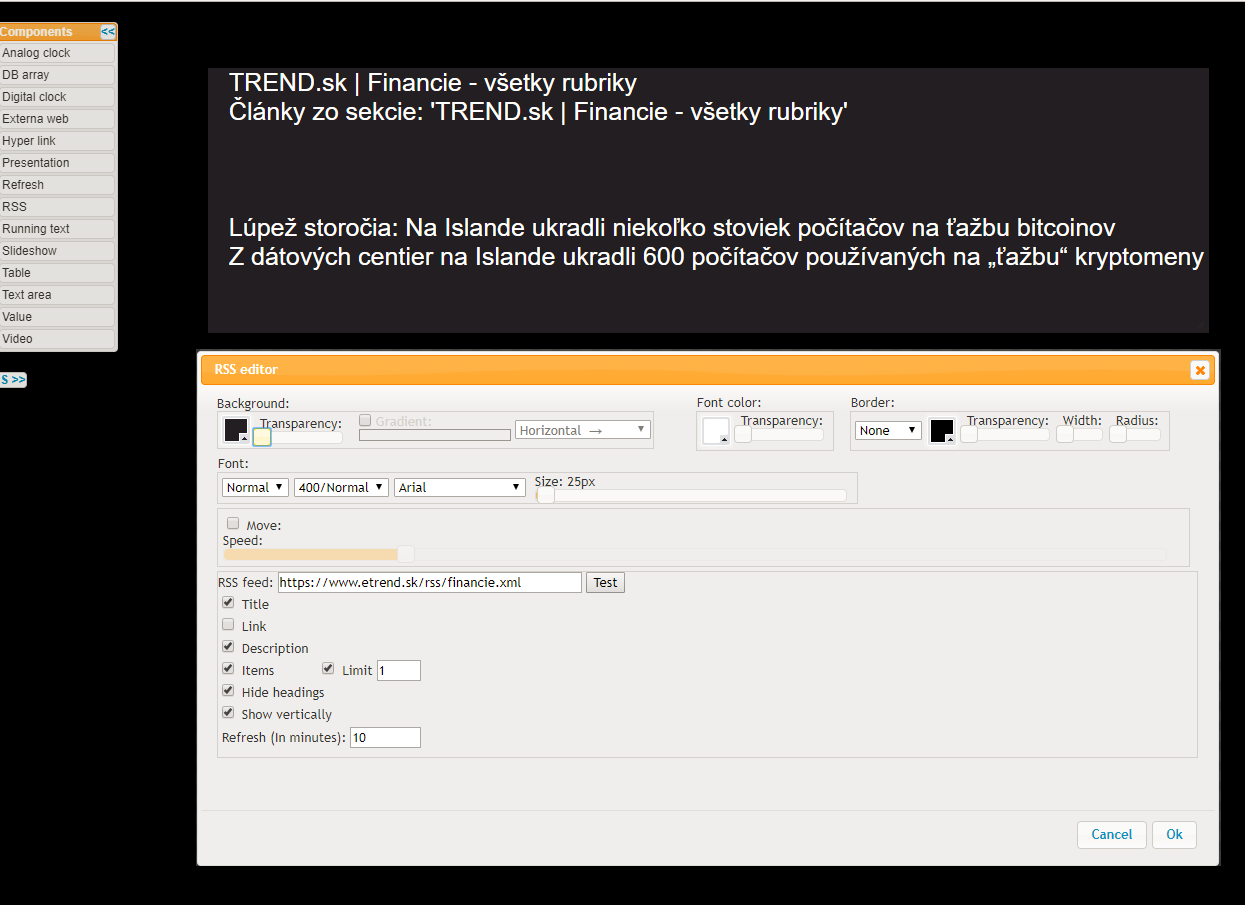
\includegraphics[width=0.85\textwidth]{RSS}
    \caption{Ukážka editora a RSS obsahu}
    \label{fig:mesh1}
\end{figure}

\subsection{Pridanie užívateľských rolí}
\textit{Zadanie:}\\
Upraviť bezpečnosť chodu aplikácie pridaním užívateľských rolí a overiť ich funkčnosť.
\begin{enumerate}
\item \textbf{Administrátor} - má možnosť pridať/editovať/vymazať panel, má možnosť pridať/editovať/vymazať stránku, má prístup k nastaveniam, môže manipulovať s časovou osou.
\item \textbf{Autor} - má možnosť pridať/editovať panel, nemôže vymazať žiadny panel, má možnosť pridať/editovať/vymazať stránku, nemá prístup k nastaveniam, môže manipulovať s časovou osou.
\item \textbf{Bežný používateľ} - nemá možnosť pridať/editovať/vymazať panel, nemá možnosť pridať/editovať/vymazať stránku, nemá prístup k nastaveniam, nemôže manipulovať s časovou osou.
\end{enumerate}
\textit{Analýza}\\
Táto požiadavka prišla od zákazníka, ktorý chcel takýmto spôsobom zvýšiť bezpečnosť chdu aplíkácie.
V prvej časti budeme musieť upraviť tabuľku \textsf{users} a pridať do nej stĺpec, ktorý nám bude vyjadrovať konkrétnu užívateľskú rolu. V ďalšej časti, bude potrebné prejsť všetky stránky a kontrollery a upraviť ich podľa zadania. 
\textit{Riešenie}\\
Postup je rozdelený do viacerých krokov. V prvom kroku budeme musieť upraviť DB model v kóde aj  pridať stĺpec do databázy. V projekte je použitý ORM nástroj Entity framework s Model first prístupom. Ten spočíva z modelovacieho nástroja, v ktorom je možné vizuálne pridávať entity , relácie a relácie medzi nimi. Tieto zmeny je následné nutné rozdielovým skriptom spustiť nad databázou. Na začiatok som sa rozhodol do projektu pridať číselník \textsf{UserRoles} , ktorý bude obsahovať  názvy rolí s číslom. Ďalej som si v modeli našiel tabuľku Users, ktorá mala niekoľko stĺpcov.  ku nim som pridal stĺpec \textsf{UserRole} s typom \textsf{Int32}. Aj napriek tomu, že v databáze je rola uložená ako číslo, Entity framework ju dokáže namapovať priamo do vytvoreného číselníka. V ďalšom kroku bolo potrebné vytvoriť rozdielový skript, ktorým zmeny premietneme do databázy.
\lstset{language=sql}
\begin{lstlisting}[caption=SQL skript pre pridanie užívateľelskej role,captionpos=b]
			ALTER TABLE [dbo.Users]
			ADD UserRole int NOT NULL DEFAULT(1)
			GO
\end{lstlisting}

V tomto prípade sme zo všetkých uživateľov spravili administrátorov. Postupne som prešiel jednotlivé záznamy v databáze a upravil skupinu podľa konkrétnych užívateľov. Pri vytvárani nových užívateľov má administrátor odteraz možnosť zvoliť skupinu novému užívateľovi.\\ Ďalšou časťou bolo prejsť všetky stránky a upraviť  niektoré časti kódu podľa skupiny prihláseného užívateľa. Mojim riešením bolo do každého modelu, ktorý sa vytvára v kontroleri a zobrazuje na stránke, pridať ďalšiu premennú, ktorú naplním užívateľovou skupinou. Tú dokážem zistiť vytiahnutím aktuálne prihláseného uživateľa z DBContextu. DBContext je brána, ktorá slúží na prístup a prácu s databázou. Na jednotlivých sránkach pomocou naplneného modelu  a razora vieme definovať , čo sa má ktorému užívateľovi zobrazovať a čo nie. Operácie ako upravovanie a vymazávanie môže robiť iba administrátor, v našom prípade užívateľská rola 1. 
\lstset{language=HTML5}
\begin{lstlisting}[caption=Zobrazenie operácii pre administrátora,captionpos=b]
<div class="buttonsPanel">
    @if(model.userRole == 1) {
    <div class="editedButtons">
        <img class="edit" src="@Url.Content("~/Content/Images/edit.png ")"
        onclick="boardmanage('@(b.Id)')" title="@Locale.GetLocaleString("edit")" />
        
        <img class="delete" src="@Url.Content("~/Content/Images/remove.png")"
         onclick="deleteBoard(@(b.Id))" title="@Locale.GetLocaleString("delete")"/>
    </div>
    }
</div>
\end{lstlisting}
\subsection*{Import udalosti do databázy}
\textit{Zadanie:}\\
Pridať možnosť importu udalostí priamo do databázy z xlsx súboru. Pridať  chybové hlásenia pri  nesprávnom formáte dokumentu a informovať používateľa o výsledku importu
\\\textit{Analýza}\\
Pri niektorých zakazníkoch sme sa streli so zaujímavou požiadavkou. Pre rýchlejšie vkladanie  udalostí na jednotlivé panely by privítali možnosť nadefinovať si ich   v tabuľkovom editore (napr. Excel) a jednoduchým spôsobom vložiť do systému. Takéto riešenie ušetrí veľa času používateľa obzvlášť pri vysokých počtoch stránok a udalostí. Zároveň pridáva možnosť  do budúcnosti vytvoriť aj export udalostí, čo by znamenalo  jednoduchý a rýchly presun z jedného systému do druhého bez zásahu administrátora alebo manuálneho vytvárania.
\\\textit{Riešenie}\\
\section{LightNet TK}
Na projekte LightNet TK som pracoval dokopy približne  30 dní. V tejto dobe  je zahrnutých aj 5 dní učenia  sa architektúry použitej vo frameworku Angular. Jednalo sa najmä o konečnú a finálnu úpravu produktu podľa potrieb zákazníka. Moja práca spočívala v úprave a vytváraní  komponentov napísaných v Typescripte a v malej miere aj práca na API  v jazyku Java s použitím technológie Spring Boot. Vďaka použitiu material design aplikácia vyzerá moderne a prehľadne.
\subsection{Pridanie šablón pre merania na rozvádzačoch }
\textit{Zadanie:}\\
Pridať do projektu grafy  z meraní. Pridať možnosť zobraziť/schovať jednotlivé inštancie  z meraní. Konečný stav môže užívateľ uložiť ako šablónu.
\\\textit{Analýza:}\\
Na stránke meraní sa nachádzajú 4 grafy  a vysoký počet inštancii v samotných grafoch,čo  je pre bežného úžívateľa pomerne zložité na rýchlu orientáciu. 
Šablóna bude uľahčovať zobrazenie grafov , ale najmä zprehľadní celú stránku od  údajov, ktoré užívateľ nepotrebuje. Táto úloha sa bude riešiť v prezenčnej vrstve - zobrazenie uživateľovi, tlačidlo na pridanie a výber šablóny . Ukladanie jednotlivých šablón bude prebiehať  na serveri, do Postgre SQL databázy.
\\\textit{Riešenie:}\\
\textbf{Klientská časť}\\
Prvým krokom bolo vymyslieť rozmiestnenie jednotlivých  tlačidiel na stránke a realizovať samotný výber šablón. To som realizoval pomocou klasického dropdown listu. V angulare môžeme tento  prvok nájsť pod názvom \lstset{language=HTML5}
\lstinline!<mat-select>!. V dropdowne budu zobrazené šablóny stiahnuté zo servera. Pre obmedzené miesto vo widgete grafov som sa rozhodol umiestniť tlačidlo na pridanie šablóny priamo do dropdown listu. Po výbere tejto možnosti sa zobrazí dialóg pre zadanie názvu šablóny. Tento dialog je realizovaný ako samotný komponent s názvom \lstset{language=HTML5}
\lstinline!MatDialog!. Po zadaní názvu sa kontroluje, či užívateľ nezadal nebezpečné symboly ako úvodzovky, pomlčky, medzeru  a podobne. V  tomto zozname tiež bude možnosť zobraziť všetky grafy a inštancie bez možnosti editácie. To je vhodné vtedy, ak úžívateľ chce mať pri vstupe na stránku zobrazené všetky údaje.  Na grafy a zobrazenie časovej osi som použil framework vis.js, ktorý podporuje rôzne druhy grafov. Medzi ďalšie dôvody patrili, že je zadarmo , jednoducho sa s ním pracuje a má rozsiahlu dokumentáciu.  Ešte pred načítaním grafov sa  najskôr zo servera načítajú všetky šablóny aktuálneho užívateľa. V Databáze je uložená aj informácia, ktorú šablónu má užívateľ predvolenú. Vďaka tomu sa zobrazia iba grafy a inštancie, ktoré užívateľ zvolil. Pri zmene  šablóny je znovu potrebné načítať dáta do grafov. a uvolniť pamäť od nepotrebných dát. Takisto bolo potrebné detekovať vypnutie nejakej inštancie grafu. Na obidve tieto udalosti som si si implementoval eventlistner, ktorý je zabudovaný v Angulari. Vďaka tomu je možné pri zmene zavolať ľubovolnú metódu. 
\lstset{language=HTML5}
\begin{lstlisting}[showstringspaces=false,caption=Dropdown pre zvolenie šablóny s využitím Two-way databinding,captionpos=b]
 <mat-select placeholder="{{"measurement_filter" | translate}}"
  [@SelectTemplateAnimation]='selectTemplateState' (change)="templateChanged()"
  [(ngModel)]="selectedTemplate" name="template" class="select-group-dropdown">
           <mat-option *ngFor="let template of templates " [value]="template">               
           </mat-option>
 </mat-select>
\end{lstlisting}

V ukážke 5.4 možete vidieť použíté viaceré nástroje Angularu, ktoré som počas  vývoja používal.
\begin{enumerate}
\item \textbf{Two-way databinding}: S touto možnosťou je možné previazať model z triedy priamo do HTML kódu. Ako názov napovedá zmeny sú obojsmerne premietnuté z HTML do modelu a naopak. V našej ukážke ho využívame v \lstset{language=HTML5}
\lstinline! [(ngModel)]="selectedTemplate"! Premenná selectedTemplate obsahuje pole objektov, ktoré sa skladajú z ID a názvu šablóny.
\item \textbf{Event binding} Vďaka event bindingu vieme pri  udalosti v HTML elemente zavolať metódu v triede komponentu. V našom prípade som sa rozhodol pri zmene šablóny (udalosť \lstinline![(change)]!) zavolať metódu \lstset{language=Javascript}
\lstinline!templateChanged()!,  ktorá inicializuje grafy  a inštancie, ktoré su zadefinované v šablóne.
\item \textbf{String interpolation} Tento nástroj umožnuje premietnuť  veci z triedy komponentu do klasického textu. Je možné takto  vypísať napríklad hodnotu premennej alebo rôzny iný text. V našej ukážke \lstset{language=Javascript}
\lstinline
[showstringspaces=false]!placeholder="{{"measurement_filter" | translate}}")! využívame String interpolation na nastavenie našeptávacieho textu. Je tu tiež použitý  tzv. piping (\textbf{|}), ktorý sa používa na ďalšiu modifikáciu textu. Napríklad zaokrúhlenie čísiel, formát dátumu, zmena textu na veľké/malé písmena a podobne. V tomto prípade  som piping použil na preklad textu, o ktorom bližšie popisujem v ďalšej kapitole.
\end{enumerate}
\textbf{Serverová časť}\\
Pri zmenách šablón bolo potrebné tieto zmeny uložiť aj do databázy. Komunákácia so serverom  prebieha  pomocou REST API. Serverová časť je napísaná v Jave technlógiou Spring boot s použitím MVC architekrúry. Vďaka tomu ostávalo  iba implementovať model a kontroler, na ktorý sa budem z klientskej časti dotazovať.
\begin{figure}[h]
    \centering
    \includegraphics[width=1\textwidth]{graphs}
    \caption{Výsledná stránka meraní }
    \label{fig:mesh1}
\end{figure}

\subsection{Lokalizácia SK/EN}
\textit{Zadanie:}\\
Lokalizovať aplikáciu do SK/EN jazyka s možnosťou výberu jazyka.
\\\textit{Analýza:}\\
Jednou z  úloh  lokalizácie bolo určiť, či sa bude vykonávať na serveri, alebo na strane klienta. Z dostupných riešení lokalizácie v rámci technoógii Spring boot a Angular  som sa rozhodol riešiť jazykovú lokalizáciu na strane klienta, v javascripte pomocou knižnice \textit{I18n}\cite{i18n}
\\\textit{Riešenie:}\\
Použitie knižnice \textit{I18n} vo framweorku angular je pomerne jednoduché. Pomocou npm si najprv nainštalujeme do projektu knižnicu.
\begin{center}
\begin{tabular}{c}
\lstset{language=HTML5}
\begin{lstlisting}[showstringspaces=false]
npm install i18n --save
\end{lstlisting}
\end{tabular}
\end{center}
Po inštalácii knižnice a  prečítaní dokumentácie  bolo  potrebné vytvoriť súbory, ktoré budú obsahovať preložené reťazce vo formáte "kľúč": "hodnota". Tieto súbory sa  musia volať podľa skratky jazyka. V mojom prípade som si v koreňovom adresári projektu vytvoril súbor \textit{sk.json} a \textit{en.json} V ďalšom kroku  bolo úlohou nájsť všetky reťazce pridať ich do  týchto súborov  aj  s preloženou hodnotou. Aby knižnica vedela, ktoré  veci sa majú prekladať je  použitý tzy. piping , s ktorým je možné meniť a upravovať textové hodnoty v HTML kóde.
\lstset{language=HTML5}
\begin{lstlisting}[showstringspaces=false,caption= String interpolation s použitím popingu na preklad,captionpos=b]
		  {{"EmailIsNotInCorrectFormat" | translate}}"
\end{lstlisting}
Knižnica sa štandardne snaží použiť jazyk, ktorý je nastavený v prehliadači. Ak sa taký jazyk  medzi vytvorenými súbormi nenachádza, ostáva ponechaná pôvodný nepreložený kľúč. Toto správanie knižnice  nevyhovovalo z viacerých dôvodov. Ku aplikácii často pristupujú aj ľudia z iných štátov a mohlo by sa ľahko stať, že sa aplikácia vôbec nepreloží, pretože neexistuje ekvivalentná jazyková verzia. Ja som sa rozhodol  nastaviť predvolený anglický jazyk a až potom podľa jazyka prehliadača  nastaviť  prípadne slovenský jazyk. Kedže knižnica je implementovaá v angulari ako služba, bolo jednoduché k nej prístúpiť v konštruktore koreňového komponentu a nastaviť jazyk. V konštruktore bolo  tiež potrbné registrovať jazykove verzie pomocou funkcie\lstset{language=JavaScript}
\lstinline!addLangs()! , ktorá berie ako parameter pole názvov jazykových verzii.
\begin{center}
\begin{tabular}{c}
\lstset{language=JavaScript}
\begin{lstlisting}[showstringspaces=false, caption=Konštruktor  aplikácie,captionpos=b]
constructor( private translateSevice: TranslateService ) {
    console.log("App created");
	
    this.translateSevice.addLangs(['en', 'sk']);
    this.translateSevice.setDefaultLang('en');
	
    let browserLang = this.translateSevice.getBrowserLang();
    this.translateSevice.use(browserLang.match(/en|sk/) ? browserLang : 'en');
}
\end{lstlisting}
\end{tabular}
\end{center}
Osobitnou kapitolou bola sránka alarmov. Alarmy predstavujú  rôzne chyby, ktoré nastali pri manipulácii s osvetlením. Každý alarm má svoj chybový kód a  chybovú správu uloženú v databáze. Úlohou bolo  pridať stĺpec ku tabuľke alarmov  s chybovou  správou v anglickom jazyku.
\subsection{Pridanie kontaktného formuláru }
\textit{Zadanie:}\\
Pridať komponent pre kontaktný formulár. Vytvoriť emailové konto a správne ho nakonfigurovať v aplikácii.
\\\textit{Analýza:}\\
Táto úloha sa dala rozdeliť zase do 2 samostatných úloh. Jednalo sa o vytvorenie formuláru, ktorý vidí užvateľ a  samostatné odoslanie emailu z hrubého klienta na adresu zadanú zákazníkom. Aby aplikácia bola schopná posielať emaily, bolo potrebné vytvoriť emailový učeť a správne ho nakonfigurovať.
\\\textit{Riešenie:}\\
Samostatný formulár sa skladá zo 6 polí(Meno odosielateľa,Spoločnosť, Adresa, Telefón, Email a Text správy) Tieto polia boli vyžiadané zakazníkom  pričom povinne vyplnené polia musia byť Meno, Email a Text správy. V angulári som si vytvoril triedu [meno], ktorá obsahovala všetky polia formuláru. Anglular obsahuje aj knižnice a mechanizmy na prácu s formulármi a ich validaciu Túto knižnicu some si museli naimportovať z  \textsf{cesta///}. Pomocou two-way databinding som načítal dáta  do inštancie tejto triedy. Potrebné validácie a pravidlá sa dajú riešiť dvomi spôsobmi. 
\begin{enumerate}
\item\textbf{Template-driven validácia} Do HTML časti  sa integrujú  atributy pre validáciu vstupov napr.: \textsf{required, minlenght, maxlenght}. Takýmto spôsobom  je niej možné formulár validovať dynamicky, čo v našom prípade ani nepotrebujeme.
\item\textbf{Reactive form validácia} Pod týmto názvom sa skrýva komplexnejšia  validácia v angular aplikáciách. Validácia sa vytvára priamo v triede komponentu pomocou funkcii.  Toto je vhodné, ak chceme validovať nejaké polia dynamicky, napríklad kontrolovať, či  zadaná emailová adresa  už nieje použitá bez odoslania formuláru.
 V našom  prípade som sa rozhodol použiť Template-driven validáciu nakoľko postačuje pre náš kontaktný formulár. Pri chybe vo validácii   bolo potrebné nastaviť tlačidlo na \textbf{disabled} aby sa predišlo odoslaniu chybného formuláru.
\begin{figure}[h]
    \centering
    \includegraphics[width=1\textwidth]{contact}
    \caption{Kontaktný formulár s ukážkou validácie }
    \label{fig:mesh1}
\end{figure}
\end{enumerate} 
 Druhou časťou bolo nájsť možnosť, ako posielať správy na email zakazníka. Bolo potrebne vytvoriť prostredníka, ktorý údaje z formuláru prepošle na email.  Ja som sa rozhodol vytvoriť emailovú schránku a nakonfigurovať ju v serverovej časti.
\subsection{Optimalizácia pre mobilné zariadenia}
\textit{Zadanie:}\\
Optimalizovať aplikáciu pre všetky mobilné zariadenia a bežne používané prehliadače.
\\\textit{Analýza:}\\
Responzivita webových stránok patrí v roku 2018 už k štandardom a moderný web sa bez nej nezaobíde. Minimálne rozlíšenie, na ktoré som sa rozhodol aplikáciu optimalizovať  bolo na šírku  350px, čo zvládné väčšina súčasných mobilných telefónov.  Samotné rozloženie  informácii z aplikácie je rozdelené to tzv. widgetov čo predstavovalo okno s plávajúcou šírkou podľa obsahu. Ďalšou úlohou bude upraviť  texty aj v hornej lište, pretože obsahuje veľký počet informácii (čas, meno prihláseného užívateľa, výber jazyka, odhlásenie)
\\\textit{Riešenie:}\\
Samotnú responzivitu som riešil  úpravou CSS tried pomocou \textsf{@media-query}, čo je funkcia, ktorá bola pridaná až vo verzii CSS3. V nej sa zadefinuje pomocou parametrov, či chceme zmeniť triedu keď je rozlíšenie väčšie alebo menšie ako zadané v parametri. Ja som sa rozhodol upravovať triedy pre 3 rôzne rozlíšenia:
\begin{enumerate}
\item \textbf{350px - 600px} - Rozlíšenie, ktoré je možné nájsť na väčšine mobilných telefónov.
\item \textbf{601px - 960px} -  Rozlíšenie, ktoré sa používa na tabletoch, poprípade na mobilných telefónoch otočených horizontálne (na šírku)
\item \textbf{960px a viac} -  Rozlíšenie použité na notebokoch a stolových počítačoch. Na tejto sekcii bolo vykonaných najmenej úprav, keďže stránka bola vyvíjaná na notebooku s takýmto rozlíšením.
\end{enumerate}
Responzivitu môžeme jednoducho simulovať použitým vývojárskych nástrojov  v prehliadači google Chrome. takýmto spôsobom som sa rozhodol používať 3 rôzne rozlíšenia z  definovaných rozsahov. Vo väčšine komponentov bolo potrebné pri malom rozlíšení zmeniť veľkosť z pixelov na hodnotu 100\%. Tým sa dosiahol efekt, že  sú čítatelné všetky texty a nič podstatné nieje skryté. Ďalším krokom bolo  pridať rozbalovacie menu. Pri malom rozlíšení sa stávalo, že údaje , ktoré boli v hornej lište  sa  do širky stránky nezmestili. Rozhodol som sa pridať ďalší kontajner, v ktorom bude zobrazené meno prihláseného používateľa a tlačidlo na odhlásenie. Tomuto  kontajnere som priradil triedu, ktorú  pomocou selektoru nastavujem na \textit{display:none;} alebo \textit{display:block;}
\begin{figure}[h]
    \centering
    \includegraphics[width=1\textwidth]{responseCompare}
    \caption{Ukážka responzivity. Neoptimalizovaná aplikácia(vľavo) a oprimalizovaná aplikácia (Vpravo) }
    \label{fig:mesh1}
\end{figure}
Takto optimalizovanú aplikáciu som skúšal po nasadení na viacerých telefónoch s viacrými prehliadačmi. Okrem úpravy CSS tried bolo potrebné na mobiloch skryť aj  bočný panel s  odkazmi na mestá a rozvádzače. To som  implementoval v konštruktore hlavného komponenta  aplikácie. Ten sa vždy zavolá pri spustení aplikácie. Keďže bočný panel je komponent tretej strany, obsahuje veľa funkcionality. Jednou z nich bolo aj funkcia \textbf{hide()}. V konštruktore  stačilo detekovať šírku stránky pomocou \textbf{window.width} Ak bola menšia ako  hodnota pre mobilny telefón( V našom prípade 600px) tak stačilo funkciu \textbf{hide()} zavolať nad panelom. 
\newpage
\subsection{Inteligentná lišta }
\textit{Zadanie:}\\
Pridať navigačnú lištu s tlačidlami a aktualnym časom. Lišta sa po posune stránky nadol skryje a po posune stránky hore sa opäť zobrazí.
\\\textit{Analýza:}\\
Inteligentnú lištu môžeme nájsť na takmer každej modernej webovej stránke. Jej úlohou je najmä zväčšiť plochu užitočných informácii na stránke, ale stále mať k dispozicii dôležité odkazy a tlačidlá  bez  zbytočného rolovania na vrch stránky. Veľký rozdiel je spoznatelný najmä pri prehliadaní stránky na mobilnom zariadení s malým rozlíšením. 
\\\textit{Riešenie:}\\
Pre túto úlohu bolo potrebné upraviť komponent \textsf{<mat-toolbar>}. Nakoľko originálny komponent neposkytuje možnosť samoschovávania lišty, bolo potrebné ju naimplementovať. Pre úpravu komponentu bolo potrebné vytvoriť triedu v kaskádvom štýle, ktorú komponentu priradím. Zároveň bolo potrebné detekovať užívateľov pohyb na stránke nahor a nadol pre zobrazenie a skrytie lišty. Pohyb  užívateľa na stránke som urobil pomocou registrácie listenera priamo v hlavnom komponente.  Pre krajší efekt a lepší UX  zážitok  som okrem posunu lišty a jej skrytia pridal do triedy  atribut na zníženie priehľadnosti \textsf{opacity:0}. Výsledkom je  lišta, ktorá sa plynulo schová po rolovaní stránky nadol. 
\lstset{language=JavaScript}
\begin{lstlisting}[showstringspaces=false, caption= Event na odchytávanie rolovania stránky,captionpos=b]
export class ScrolllistenerDirective implements AfterViewInit {
  @Output() scrolledUp: EventEmitter<any> = new EventEmitter();
  @Output() scrolledDown: EventEmitter<any> = new EventEmitter();
  public scrollEvent: Subject<any> = new Subject();

  private currentScroll = 0;

  @HostListener('scroll', ['$event'])
  onScroll(e) {
    let el = e.target;
    let value = e.target.scrollTop;
    if (value > this.currentScroll) {
      this.scrolledDown.emit();
      this.scrollEvent.next("scrolledDown");
    }
    else if (value < this.currentScroll) {
      this.scrolledUp.emit();
      this.scrollEvent.next("scrolledUp");
    }
    this.currentScroll = value;

  }
\end{lstlisting}

\section{Správa evidencie operátorov - OAC}
Správa evidencie operátorov - OAC  je jeden z prvých projektov, ktorý beží na novej propietárne vyvinutej platforme. Súčasne so vznikom  novej platformy prebiehalo aj odlaďovanie chýb  a implementácia nových vecí v platforme. Jedná sa o ASP.NET webov0 stránky napísané v jazyku C\#. Ako ORM nástroj  bol použitý Entity framework s prístupom code-first. Vďaka tomu je možné riadiť verziu  databázy pomocou migrácii, ktor0 sa p93u priamo v C\# kóde. Projekt je vyvíjaný podľa architektúry MVC, ktorá oddeluje rôzne vrstvy systému. Súčasne s MVC architekrúrou boli použité aj ďalšie návrhové vzory. 

\subsection{Platforma - Property  comparator}\label{sssec:num1}
\textit{Zadanie:}\\
Vytvoriť atribút na porovnávanie property v rámci jedného modelu.
\\\textit{Analýza:}\\
Medzi väčšie  úlohy, ktoré  bolo potrebné implementovať na úrovni platformy bolo vytvorenie atributu pre porovnávanie polí vo formulári. Táto úloha nie je  závislá iba na projekte, ale  jej využitie sa môže hodiť aj na iných projektoch, ktoré budú bežať na platforme. V MVC architekrúre sa validácia implementuje priamo v modeli pomocou rôznych atribútov. Napríklad či je pole povinné, alebo nie, minimálna alebo maximálna dĺžka reťazca, alebo číselný rozsah. Pre zníženie záťaže servera je možné zapnúť aj klientskú validáciu, kedy sa formulár overuje priamo v javascripte. Ak formulár nieje  validný, na server sa neodošle a tým pádom ho server nemusí ďalej spracovávať. Validácia  na serveri ale nemôžeme úplne vypnúť, pretože klient  má plnú kontrolu nad kódom v javascripte a po  úprave môže obísť validáciu poslať aj formulár, ktorý nie je validný. V projekte používame teda dvojitú validáciu. Pod zadnaím úlohy sa rozumie vytvoriť atribút, ktorý sa bude správať ako validátor polí. V jeho konštruktore  sa bude prijmať názov druhého poľa, ku ktorému bude porovnávaný a operátor. Takýmto komparátorom je možné napríklad  overovať hodnoty napr. začiatok musí byť menš ako koniec, alebo hodnota v jednom poli musí byť menšia ako v druhom poli a podobne. Súčasne bude potrebné implementovať validáciu aj na strane klienta, aby sa  formulár s nesprávnymi dátami zbytočne neposielal na server.
\\\textit{Riešenie:}\\
Na začiatok som si vytvoril triedu, ktorá implmenetuje rozhranie ??? . Nad samotnou triedu je potrebné zadefinovať atribút, aby bolo jasné nad akým typom sa tento vytvorený atribút môže používať. Ja  potrebujem porovnávať iba hodnoty vrámci jednej triedy (modelu)  a preto  som nastavil na triedu atribút [blabl??]. Trieda musí implementovať rozhranie ?? . Všetky triedy rozhrania treba prepísať vlastnou funkcionalitou.  V prvom kroku  treba ytvoriť validáciu na strane servera. V konštruktore atribútu nie je možné dať ako parameter inú propertu. Súčasne so vznikom atribútu však vieme zistiť v ktorej triede sa práve aplikuje. Vieme zistiť jej názov, typ a pristupovať  k jednotlivým propertám. Ja som sa kvôli jednoduchosti rozhodol ako argument poslať reťazec s názvom druhej property.  Pre prípad, keď by sa náhodou premenovala ,  kompilátor by nhlsil žiadnu chybu, pretože ju berie ao reťazec. Toto môžeme vyriešiť náhradou reťazca príkazom  nameof(<druhyfield>) . Tym zarucime, ze aj ked sa  náhodou premenuje , koplikátor nám okamžite podčiarkne chybu, lebo taký názov nepozná. V parametroch bolo potrebné ďalej zadať operátor , pre aký sa ma vyhodnocovať validácia ako správna. To som vyriešiť vytvorením enumu, kde sú základné porovnávacie operácie (<, >, ==, <=, >=). Teraz už vieme , pristupovať k propertám triedy a vieme na základe čoho ich chceme porovnávať. Samotné overovanie  validity modelu sa vykonáva až vo funkcii ??? .  
\subsection{Implementácia business logiky}
\textit{Zadanie:}\\
Implementovať projektovú business logiku na správu pozícií a produkčných modelov.
\\\textit{Analýza:}\\
Pre oddelenie business logiky od kontrolerov a pre prácu s databázou je v projekte použitý návrhový vzor \textbf{Repozitár}. V projekte je vytvorený repozitár pre každú entitu, čím  sprehľadnuje celú aplikáciu a sústreduje všetky metódy na prístup do databázy na jedno miesto v rámci entity. Ďalší návrhový vzor je \textbf{Unit OF Work}. Ten sa stará o to, aby každú malú operáciu nebol nutný zásah do databázy. Predstavme si situáciu, keď v jedne sitácii chceme  naríklad  vymazať 50 entít a pridať ďalších 50 v jednej akcii. Unit of work zabezpečuje to, že tieto zmeny sú najskôr uložené  iba v pamäti a až v závere akcie sa tieto zmeny premietnu do databázy funkciou \textit{Commit()}
\\\textit{Riešenie:}\\
\subsection{Formulár na pridanie pozície}
\textit{Zadanie:}\\
Vytvoriť formulár na pridanie a editáciu pozícii podľa projektovej dokumentácie.
\\\textit{Analýza:}\\
Projekt sa z veľkej miery skladá z rôznych formulárov na editáciu a pridávanie  dát do databázy. Jednou z úloh, ktoré mi boli pridelené bolo aj vytvorenie formuláru a pridanie pozície. Pozícia je entita, na ktorá  predstavuje nejaké  fyzické miesto  v hale. Je previazaná s ďalšími entitami: produkčný model a ???. Mojou úlohou bude  vytvoriť model pohľad (view) a  implementovať  metódu v kontroleri, ktorá bude dáta  spracovávať. 
\\\textit{Riešenie:}\\
V prvom kroku, som si vytvoril model v priečinku, kde sú ostatné modely projektu. Tento model obsahuje  všetky polia, ktoré sa nachádzajú aj v entite. Nad každé pole je možné zadať rôzne atribúty. V mojom prípade som použil atribúty \textbf{[Required]} , ktorý značí, že pole  musí byť vyplnené nejakou hodnotou a \textbf{[MaxLength(512)]}a \textbf{[MaxLength(64)]} , ktoré značia maximálny počet znakov v textovom reťazci. Okrem štandardných atribútov na validáciu bolo potrebné aj validovať  správnosť IPv4 adresy. Na to som použiil regulárne výrazy, ktoré C\# štandardne podporuje. V tomto modeli sa nachádzali aj dve polia, ktoré bolo potrebné porovnať medzi sebou. Z dokumentácie projektu vyplývalo , že pole \textit{Pracovný čas} musí byť menšie ako pole \textit{Max. pracovný čas}. Na toto sa  dá využiť platoformový property komparátor, na ktorom som pracoval ako na samostatnej úlohe. Bližšie je o ňom  je popísané v časti \ref{sssec:num1}
\lstset{language=C++}
\begin{lstlisting}[showstringspaces=false, caption= Časť modelu pozície s validačnými atribútmi,captionpos=b]
 public class PositionModel
 {        
        [RegularExpression(@"^((25[0-5]|2[0-4][0-9]|[01]?[0-9][0-9]?)\.)
        {3}(25[0-5]|2[0-4][0-9]|[01]?[0-9][0-9]?)$", 
        ErrorMessage ="Not valid IPv4 address")]
        [Display(Name = "IPAddress", ResourceType = typeof(PositionLocale))]
        public string IPAddress { get; set; }

        [Required]
        [M2MSComparator(CompareOperator.LESS_THAN, nameof(MaxWorkDuration))]
        [DataType("TimeSpan")]
        [Display(Name = "WorkDuration", ResourceType = typeof(PositionLocale))]
        public TimeSpan WorkDuration { get; set; }

        [Required]
        [M2MSComparator(CompareOperator.MORE_THAN, nameof(WorkDuration))]
        [DataType("TimeSpan")]
        [Display(Name = "MaxWorkDuration", ResourceType = typeof(PositionLocale))]
        public TimeSpan MaxWorkDuration { get; set; }
        
        [StringLength(512)]
        [Display(Name = "Description", ResourceType = typeof(PositionLocale))]
        [DataType(DataType.MultilineText)]
        public string Description { get; set; }        
 }
\end{lstlisting}
\section{Navigácia v budovách - analáyza}
Navigácia je v sučasnosti veľmi rozsiahlou problematikou , o ktorej by sa dala napísať samotná bakalárka práca. Moderné systémy ako napríklad GPS  sú najpoužívanejšie a najznámejšie. Fungujú  na základe odozvy signálu z niekoľkých satelitov , ktoré sa voľne pohybujú vo vesmíre.  GPS systém  má však podstatnú nevýhodu - priechod signálu cez prekážku. Ak by sme chceli použiť GPS signál  napríklad v podzemí alebo v budove, signál by sme  chytili iba veľmi sporadicky, alebo dokonca vôbec. Firma, v ktorej som vykonával prax sa venuje najmä priemyselným riešeniam. Jednou z akvizícii bolo  aj navigovanie  a lokalizácia v priestore - najmä v výrobných  halách a skladoch. Mojou úlohou bolo skúsiť  nájsť všetky dostupné riešenia  s detailnou analýzou. Okrem toho bolo mojou úlohou skúsiť zbierať  dáta zo senzorov mobilu(Akcelerometer, gyroskop a magnetometer)  a analyzovať ich, či je možné z nich získať  absolútnu pozíciu bez použitia GPS systému. Celá akvizícia je iba vo veľmi počiatočnej fáze  analýzy a preto ju spomínam iba veľmi okrajovo. 

\subsection{Porovnanie dostupných technológii}
Mojou prvou úlohou bolo nájsť a  porovnať všetky dostupné technológie , ktoré  by sa potenciálne mohli použiť na navigáciu v budových bez použitia GPS systémov. V analýze by mali byť zahrnuté  výhody, nevýhody,  technológia , analýza ceny, presnosť a podobne. Všetky informácie som čerpal z internetových zdrojov a rôznych videí. Ja som sa rozhodol o každej technológii  v krátkosti popísať a najdôležitejšie informácie zhrnúť do tabuľky. (\ref{tab})
\begin{itemize}
\item\textbf{Magneticke pole} Technológia je založená na  meraní úrovne magnetického poľa. Vychádza z toho, že každé miesto v budove má jedinečnú hodnotu magnetického poľa a je možne na základe tejto hodnoty určit   približnu lokáciu. Tento systém je možné použiť v budovách, kde nedochádza k  presunu nábytku a  veľkých predmetov ako nákupné centrá a nemocnice. Pre použitie v priemysle a v skladoch  s častým presúvaním rôznych kovových predmetov  a pohybom okolo silných elektromotorov je tento systém nepoužiteľný.
\item\textbf{BLE beacony} V súčasnosti patrí jedno k najpoužívanejším  lokalizačným systémom  bez použitia GPS. Technológia pozostáva  s rozmiestnením bluetooth zariadení po budove a meraním útlmu signálu  napríklad mobilom. Pre zvýšenie životnosti týchto zariadení sa zvyčajne používa štandard BLE (\textit{Bluetooth Low Energy}), ktorý je v potovostnom režime a aktivuje sa iba pri požiadavke na komunikáciu. Pri  zistené úrovni signálu z  3 rôznych zariadení je možné pomocou trilaterácie vypočítať približnú polohu. Zariadenie je šak veľmi náročné z hľadiska počiatočnej aj dlhodobej  ceny. Pri výrobnej hale  100x100m by bolo potrebné použiť minimálne 100 Bluetooth zariadení. Každé zariadenie potrebuje inštaláciu a prívod napájania, čo predstavuje vysoké náklady pre zákazníka. 
\item\textbf{Wifi} Vychádza z podobnýh princípov ako BLE beacony. Jediným rozdielom je to, že je možné použiť už existujúcu infraštruktúru wifi access pointov v budovách. Veľkou nevýhodou je citlivosť na prekážky a nedostatočná presnosť.
\item\textbf{UWB} Ultra wideband je  pomerne nová technológia , ktorá je  navrhnutá pre vyriešenie problémov , ktoré vznikajú pri predchádzajúcich riešeniach. Tým , že pracuje na  vysokej frekvencii 3GHz až 10GHz, so šírkou pásma až 500MHz dokáže  bez problémov prejsť aj prekážkami a stenami bez zníženia presnosti. Výrobcovia technológie úvádzajú veľmi vysokú presnosť, ktorá však v reali dosahuje nižšie výsledky presnosti. Medzi jej nevýhodý patrí najmä vysoká cena zariadené a limitujúci maximálny počet  navigovaných objektov v počte približne 10 objektov.
\item\textbf{Akcelerometer} Na požiadanie mojho šéfa Martina som dostal za úlohu preskúmať  aj  možnosť využiť   senzory z mobilu ako navigáciu. Jej výhody by mali plynúť z jednoduchosti použitia , vyhnutiu sa vybudovaniu infraštruktúry  a nízkej ceny inštalácie. Na zistovanie pohybu   je použitelný  akcelerometer. Ten zbiera údaje o zrýchlení v jednotkách \textit{m/s\textsuperscript{2}}. Podľa teórie, by sme mali byť schopní prvým integrálom vypočítať rýchlosť a druhým integrálom prejdenú vzdialenosť. Aj pri pomerne zložitých výpočtoch a zašumenému signálu zo senzoru padlo na prvotné rozhodnutie  začať zbierať dáta z akcelerometra.
\end{itemize}

\begin{table}
\centering
\label{tab}
\begin{tabular}{|l|c|c|c|c|c|}
\hline
                              & \textbf{Mag. pole} & \textbf{BLE beacony} & \textbf{Wifi} & \textbf{UWB}  & \textbf{Akcelerometer} \\ \hline
\textbf{Presnosť}             & 1-2.8m                        & 2m                         & 4m            & \textless30cm & Veľmi nepresné            \\ \hline
\textbf{Dosah}                & -                             & 10m                        & 15m           & 25m           & -                         \\ \hline
\textbf{Vstupná investícia}   & Veľmi nízka                   & Veľmi vysoká               & Nízka         & Veľmi vysoká  & Veľmi nízka               \\ \hline
\textbf{Cena za údržbu}       & Nízka                         & Veľmi zložitá              & Nízka         & Veľmi vysoká  & Veľmi nízka               \\ \hline
\textbf{Zložitosť inštalácie} & Nízka                         & Veľmi zložitá              & Zložitá       & Zložitá       & Žiadna                    \\ \hline
\end{tabular}
\caption{Porovnanie  jednotlivých technológií}
\end{table}

\subsection{Zber dát zo senzorov  v mobile}
Po  prvotnej analýze nasledovalo aj napriek prevyšujúcim nevýhodam možnosť zbierať dáta z akcelerometre

\subsection{Implementácia Kalmanovho filtra}
Po úspešnom zozbieraní dát prišla na rad ich analýza a výpočty. Hneď na začiatku bol oz grafu vidieť, že signál je značne zašumený, čo môže  výrazne ovplyvniť  výsledok. 

\newpage	
\chapter{Záver}
blabla ä
\begin{table}[h!]
\centering
\begin{tabular}{|c | c | c | c|} 
 \hline
  & Počet hodín & Počet dní\\ [0.5ex] 
 \hline
 Infopanely & 56 & 7  \\ 
Lightnet TK & 220 & 27  \\
Správa operátorov - OAC & 150 & 19  \\
 Navigácia v budovách - analýza& 50 & 6   \\
 \hline
\end{tabular}
\caption{Odpracovaný čas na jednotlivých projektoch}
\end{table}

%\backmatter

\newpage
\thispagestyle{empty}
\nocite{*}
\clearpage

\printbibliography

\end{document}


